\documentclass[10pt, aspectratio=169]{beamer}

\usepackage{fontspec}
\usetheme{metropolis}
\usepackage{appendixnumberbeamer}

\metroset{titleformat frame=smallcaps}

\definecolor{cadmiumgreen}{rgb}{0.0, 0.42, 0.24}

\title{Zephyr in Action}
\subtitle{Real-World Product Development - An Interactive Workshop}
\date{\today}
\author{Jonas Remmert, Phytec Messtechnik GmbH}

\begin{document}

\maketitle

\begin{frame}{Table of contents}
  \setbeamertemplate{section in toc}[sections numbered]
  \tableofcontents[hideallsubsections]
\end{frame}

%******************************************************************************
\section{Getting Started}

\begin{frame}[fragile]{What is Zephyr?}

  \begin{columns}

    \begin{column}{0.6\textwidth}
      \begin{block}{An RTOS for IoT}
        \begin{itemize}
          \item multiple supported architectures (ARM, RISC-V, x86...)
          \item Multi-threading
          \item Power Management
        \end{itemize}
      \end{block}
      \begin{block}{and much more!}
        \begin{itemize}
          \item Open Source Bluetooth Low Energy Stack
          \item Networking, USB, Filesystems, Cryptography
          \item Shell, Logging, Sensors, Display, Audio
        \end{itemize}
      \end{block}
      \begin{block}{Ideal to build IoT products}
        \begin{itemize}
          \item Well supported for a wide range of hardware
          \item Vendor neutral steering by Linux Foundation
          \item Coding Style and Concepts from the Linux Kernel
        \end{itemize}
      \end{block}
    \end{column}

    \begin{column}{0.4\textwidth}
      \begin{figure}
        
\includegraphics[width=0.73\textwidth]{images/zephyr_logo.png}
      \end{figure}
    \end{column}

  \end{columns}
\end{frame}

\begin{frame}[fragile]{How to get started?}

  \begin{block}{Documentation}
    \begin{itemize}
      \item Documentation: {\scriptsize \url{https://docs.zephyrproject.org/latest/}}
      \item Getting Started Guide: {\scriptsize \url{https://docs.zephyrproject.org/latest/develop/getting_started/}}
      \item Supported Boards: {\scriptsize \url{https://docs.zephyrproject.org/latest/boards/}}
      \item Samples and Demos: {\scriptsize \url{https://docs.zephyrproject.org/latest/samples/}}
    \end{itemize}
  \end{block}
  \begin{block}{Source}
    \begin{itemize}
      \item Zephyr source (GitHub): {\scriptsize \url{https://github.com/zephyrproject-rtos/zephyr}}
      \item Out-of-tree application example: {\scriptsize \url{https://github.com/zephyrproject-rtos/zephyr}}
    \end{itemize}
  \end{block}
\end{frame}

%******************************************************************************
\section{Setting up the Development Environment}

\begin{frame}[fragile]{Setting up the Development Environment}

  \begin{block}{Types of Requirements}
    \begin{itemize}
      \item Linux, macOS or Windows 10/11
      \item Installation Requirements (CMake, Python3..)
      \item Python Requirements (west, pyocd..)
      \item Zephyr SDK that provides Toolchains (gcc, gdb, newlib..)
    \end{itemize}
  \end{block}
  Everything is described in the Zephyr Getting Started Guide.
\end{frame}

%******************************************************************************
\section{Samples, Applications and Products}

\begin{frame}[fragile]{Samples in Zephyr}

  \begin{block}{Samples}
    \begin{itemize}
      \item Zephyr provides a wide range of samples
      \item Samples are located in \texttt{zephyr/samples/}
      \item Isolated functionality or feature
    \end{itemize}
  \end{block}
  \begin{block}{Tests}
    \begin{itemize}
      \item Tests are located in \texttt{zephyr/tests/}
      \item Isolated test cases for a feature or hardware
      \item Useful to test e.g. a device driver
    \end{itemize}
  \end{block}
  \begin{block}{Applications}
    \begin{itemize}
      \item ZSWatch - Open Source Smart Watch: {\scriptsize \url{https://github.com/jakkra/ZSWatch}}
    \end{itemize}
  \end{block}
\end{frame}

\begin{frame}[fragile]{Why Zephyr for products}

    TBD: Reasons for Zephyr in Products

  \begin{block}{Examples}
    \begin{itemize}
       \item Overview: {\scriptsize \url{https://www.zephyrproject.org/products-running-zephyr/}}
       \item Wildlife Tracking and Protection (OpenCollar)
       \item Wind Turbines (Vestas)
       \item Hearing Aid (Oticon)
       \item Wastewater Pump Monitoring (BeST Sensor, German Railways - DB)
    \end{itemize}
  \end{block}
\end{frame}

%******************************************************************************
\section{Hands-on Examples}

\begin{frame}[fragile]{Examples for this Workshop}

  Five different examples that show a (small) subset of Zephyr features.

  \begin{block}{Examples}
    \begin{enumerate}
       \item Hello World
       \item Logging
       \item Workqueues (and runtime context)
       \item Shell
       \item Sensor
       \item Bluetooth Low Energy
    \end{enumerate}
  \end{block}
\end{frame}

\begin{frame}[fragile]{01\_hello\_world}

  \begin{itemize}
     \item Structure of a Zephyr Application
     \item Zephyr Repository: \texttt{zephyr/samples/hello\_world}
  \end{itemize}

  \begin{columns}[T,onlytextwidth]
    \column{0.5\textwidth}
      \begin{block}{Build}
        \begin{itemize}
          \item {\scriptsize west build -b qemu\_cortex\_m0 samples/01\_hello\_world -p}
        \end{itemize}
      \end{block}

     \begin{block}{Run}
        \begin{itemize}
          \item {\scriptsize west build -t run}
        \end{itemize}
      \end{block}

    \column{0.5\textwidth}

      \metroset{block=fill}

      \begin{exampleblock}{Expected terminal output}

        {\fontsize{7}{9.6}\selectfont
          \begin{verbatim}
*** Booting Zephyr OS build zephyr-v3.4.0 ***
Hello World! qemu_cortex_m0
          \end{verbatim}
        }
      \end{exampleblock}
  \end{columns}
\end{frame}


\begin{frame}[fragile]{02\_logging}

  \begin{itemize}
     \item Logging API
     \item Zephyr Repository: \texttt{zephyr/samples/subsys/logging}
  \end{itemize}

  \begin{columns}[T,onlytextwidth]
    \column{0.5\textwidth}
      \begin{block}{Build}
        \begin{itemize}
          \item {\scriptsize west build -b qemu\_cortex\_m0 samples/02\_logging}
        \end{itemize}
      \end{block}

     \begin{block}{Run}
        \begin{itemize}
          \item {\scriptsize west build -t run}
        \end{itemize}
      \end{block}

    \column{0.5\textwidth}

      \metroset{block=fill}

      \begin{exampleblock}{Expected terminal output}

        {\fontsize{6}{9.6}\selectfont
          \begin{verbatim}
 *** Booting Zephyr OS build zephyr-v3.4.0 ***
Hello World! qemu_cortex_m0
[00:00.001,570] <err> hello_world: error str
[00:00.001,593] <dbg> hello_world: main: debug str
[00:00.001,605] <inf> hello_world: info str
[..]
          \end{verbatim}
        }
      \end{exampleblock}
  \end{columns}
\end{frame}


\begin{frame}[fragile]{02\_workqueues}

  \begin{itemize}
     \item Work items getting called from a queue
     \item Offload work from interrupt context
  \end{itemize}

  \begin{columns}[T,onlytextwidth]
    \column{0.5\textwidth}
      \begin{block}{Build}
        \begin{itemize}
          \item {\scriptsize west build -b qemu\_cortex\_m0 samples/03\_workqueues}
        \end{itemize}
      \end{block}

     \begin{block}{Run}
        \begin{itemize}
          \item {\scriptsize west build -t run}
        \end{itemize}
      \end{block}

    \column{0.5\textwidth}

      \metroset{block=fill}

      \begin{exampleblock}{Expected terminal output}

        {\fontsize{6}{9.6}\selectfont
          \begin{verbatim}
 *** Booting Zephyr OS build zephyr-v3.4.0 ***
Hello World! qemu_cortex_m0
[00:00.001,570] <err> hello_world: error str
[00:00.001,593] <dbg> hello_world: main: debug str
[00:00.001,605] <inf> hello_world: info str
[..]
          \end{verbatim}
        }
      \end{exampleblock}
  \end{columns}
\end{frame}


\begin{frame}[fragile]{04\_shell}

  \begin{itemize}
     \item Interactive Shell with user-defined commands
     \item Zephyr Repository: \texttt{zephyr/samples/subsys/shell/shell\_module}
  \end{itemize}

  \begin{columns}[T,onlytextwidth]
    \column{0.5\textwidth}
      \begin{block}{Build}
        \begin{itemize}
          \item {\scriptsize west build -b qemu\_cortex\_m0 samples/04\_shell -p}
        \end{itemize}
      \end{block}

     \begin{block}{Run}
        \begin{itemize}
          \item {\scriptsize west build -t run}
          \item {\scriptsize -> press "tab" to show commands}
        \end{itemize}
      \end{block}

    \column{0.5\textwidth}

      \metroset{block=fill}

      \begin{exampleblock}{Expected terminal output}

        {\fontsize{7}{9.6}\selectfont
          \begin{verbatim}
uart:~$ 
  bypass              clear
  date                demo
  device              devmem
  dynamic             help
  history             kernel
  log                 log_test
  nrf_clock_control   resize
  retval              section_cmd
  shell               shell_uart_release
  stats               version
          \end{verbatim}
        }
      \end{exampleblock}
  \end{columns}

\end{frame}

\begin{frame}[fragile]{04\_shell}

  \metroset{block=fill}
\begin{exampleblock}{List of threads running on the system (shortened)}

    {\fontsize{7}{9.6}\selectfont
      \begin{verbatim}
uart:~$ kernel threads 
Threads:
 0x200008a0 sysworkq  
	options: 0x0, priority: -1 timeout: 0
	Total execution cycles: 137 (0 %)
	stack size 1024, unused 856, usage 168 / 1024 (16 %)

*0x20000390 shell_uart
	options: 0x0, priority: 14 timeout: 0
	Total execution cycles: 144111 (0 %)
	stack size 2048, unused 896, usage 1152 / 2048 (56 %)

 0x200006b0 idle
	options: 0x1, priority: 15 timeout: 0
	Total execution cycles: 588177458 (99 %)
	stack size 256, unused 164, usage 92 / 256 (35 %)
      \end{verbatim}
    }
  \end{exampleblock}

\end{frame}

\begin{frame}[fragile]{05\_sensor}

  \begin{itemize}
     \item TI HDC1010: I2C Temperature and Humidity Sensor
     \item Zephyr repository: \texttt{zephyr/samples/sensor/ti\_hdc/}
  \end{itemize}

  \begin{columns}[T,onlytextwidth]
    \column{0.45\textwidth}
      \begin{block}{Build}
        \begin{itemize}
          \item {\scriptsize west build -b reel\_board samples/05\_sensor -p}
        \end{itemize}
      \end{block}

     \begin{block}{Flash}
        \begin{itemize}
          \item {\scriptsize west flash}
        \end{itemize}
      \end{block}

     \begin{block}{Show Terminal output}
        \begin{itemize}
           \item {\scriptsize reel board is connected via USB-Serial}
           \item {\scriptsize Check serial device (tty dev/com port)}
           \item {\scriptsize connect to board via terminal (minicom, tio,..)}
        \end{itemize}
      \end{block}

    \column{0.55\textwidth}

      \begin{exampleblock}{Expected terminal output (shortened)}
      \metroset{block=fill}
        {\fontsize{7}{9.6}\selectfont
          \begin{verbatim}
*** Booting Zephyr OS build zephyr-v3.4.0 ***
Running on arm!
Dev 0x8584 name ti_hdc@43 is ready!
Fetching...
Temp = 26.356506 C, RH = 59.747314 %
Fetching...
Temp = 26.406860 C, RH = 59.149169 %
          \end{verbatim}
        }
      \end{exampleblock}
  \end{columns}

\end{frame}

\begin{frame}[fragile]{06\_ble}

  \begin{itemize}
     \item BLE Peripheral device, temperature monitor
     \item Zephyr repository: \texttt{zephyr/samples/bluetooth/peripheral\_ht}
     \item App to connect: nRF Connect for Mobile (Android, iOS)
  \end{itemize}

  \begin{columns}[T,onlytextwidth]
    \column{0.45\textwidth}
      \begin{block}{Build}
        \begin{itemize}
          \item {\scriptsize west build -b reel\_board samples/06\_ble -p}
        \end{itemize}
      \end{block}

     \begin{block}{Flash}
        \begin{itemize}
          \item {\scriptsize west flash}
        \end{itemize}
      \end{block}

     \begin{block}{Show Terminal output}
        \begin{itemize}
	  \item {\scriptsize reel board is connected via USB-Serial}
	  \item {\scriptsize Check serial device (tty dev/com port)}
	  \item {\scriptsize connect to board via terminal (minicom, tio,..)}
        \end{itemize}
      \end{block}

    \column{0.55\textwidth}

      \begin{exampleblock}{Expected terminal output (shortened)}
      \metroset{block=fill}
        {\fontsize{7}{9.6}\selectfont
          \begin{verbatim}
*** Booting Zephyr OS build zephyr-v3.4.0 ***
bt_hci_core: HW Platform: Nordic Semiconductor
bt_hci_core: HW Variant: nRF52x
bt_hci_core: Firmware: Standard BT controller 3.4
bt_hci_core: Identity: CC:42:FB:73:2F:36 (random)
bt_hci_core: HCI: version 5.4 rev 0x0000, mfg 0x05f1
bt_hci_core: LMP: version 5.4 subver 0xffff
Bluetooth initialized
temp device is 0x26500, name is temp@4000c000
Advertising successfully started
          \end{verbatim}
        }
      \end{exampleblock}
  \end{columns}

\end{frame}

\begin{frame}[fragile]{06\_ble - Connect to device via 'nRF Connect for Mobile'}

  \begin{columns}[T,onlytextwidth]
    \column{0.30\textwidth}

      \begin{exampleblock}{Terminal output}
      \metroset{block=fill}
        {\fontsize{7}{9.6}\selectfont
          \begin{verbatim}
[..]
Connected
temperature is 28C
Indication success
Indication complete
          \end{verbatim}
        }
      \end{exampleblock}

    \column{0.30\textwidth}
      \begin{figure}
        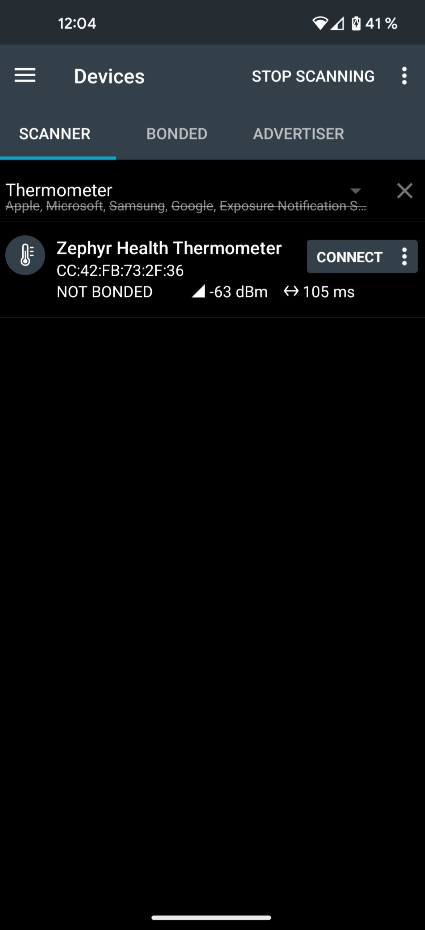
\includegraphics[width=0.8\textwidth]{images/nrf_connect_scan.png}
      \end{figure}
    \column{0.30\textwidth}
      \begin{figure}
        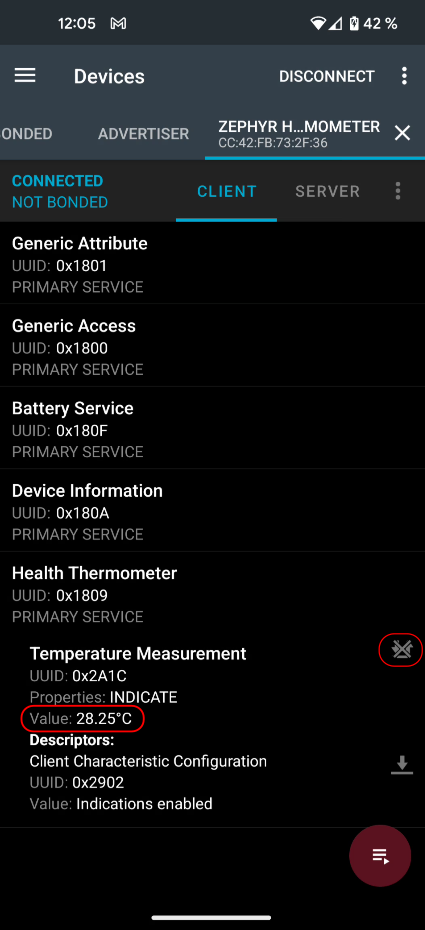
\includegraphics[width=0.8\textwidth]{images/nrf_connect_ble_connected.png}
      \end{figure}


  \end{columns}

\end{frame}

%*****************************************************************************
\begin{frame}[standout]
  Questions?
\end{frame}

\end{document}
